\documentclass{article}
\usepackage{graphicx} % Required for inserting images

\title{Clase 2: Modo Matemático}
\author{Daniel Sánchez}
\date{January 2025}

\usepackage{amsmath} % para dfrac y simbolos
\usepackage{csquotes} % para comillas rapidas\
\usepackage{booktabs} % lineas para tablas
\usepackage{hyperref}
\usepackage{float}
\usepackage{lipsum}
\usepackage[spanish]{babel}

\begin{document}

\maketitle % Hacer titulo

\tableofcontents

\listoffigures

\listoftables

\clearpage

\lipsum

\section{Sintaxis de modo matematico en \LaTeX}

\subsection{sintaxis basica}

Entrar a modo matematico con signo de dolar \$: (doble signo de dolar para display \$ \$)

\begin{enumerate}
    \item Exponentes: \textasciicircum (sombrero): $x^2 + 1 - 2 + 3$ 
$$ x^2 + 1 - 2 +3$$
    \item Subindices: guion bajo: $x_i$

$$x_i$$
    $$x_i^5$$
    \item Fraccion (comando frac): $\frac{1}{2}$ (inline fraction)
    \item Fraccion display (comando dfrac) $\dfrac{1}{2}$ (display frac)
    \item Raiz cuadrada (sqrt): $\sqrt{2}$
    \item Raiz de cualquier n: $\sqrt[3]{2}$. en llaves va lo que esta debajo de la raiz y en corchetes (opcional) va lo que esta arriba. 
    \item Exponente “avanzado”: $x^{15}$, $x^{\frac{5}{2}}$, aplica lo mismo para exponentes. 

\enquote{comillas}

"hola"

\end{enumerate}


\subsection{simbolos}

$\beta$

$\alpha$

$\Delta$

$\delta$

$\varepsilon$

$\epsilon$

\begin{equation}
  \min_{\beta} \sum_{i=1}^{n} (y_i - \beta_0 - \beta_1 x_{i1} - \beta_2 x_{i2} - \cdots - \beta_k x_{ik})^2
  \label{eq:ols_optimization}
\end{equation}

Simbolos de operaciones matematicas

$log$ (no)

$\log(x)$

$\text{log}$

$\log(\text{ingresos})_i = \beta_0 + \beta_1 \text{educacion}_i + \varepsilon_i$

$min$ (no)

$\min$

$\max$

$$\displaystyle \sum_{i=1}^n x_i$$

$$\displaystyle \int_i^j x \ dx$$

\subsection{alineaciones}

\begin{equation*}
    \log(\text{ingresos})_i = \beta_0 + \beta_1 \text{educacion}_i + \varepsilon_i
\end{equation*}

asterisco para no enumerar. 

\begin{align*}
    y &= \beta_0 + 1 \\
    y &= \beta_0 + \beta_1 + 1 
\end{align*}

Alinear varios bloques de ecuaciones. Usar doble \&\&:

\begin{align*}
    y &= \beta_0 + 1 && y = \beta_0 + \beta_1 + 1 \\
    y &= \beta_3 + 7 && y= \beta_3 + \beta_{10}
\end{align*}

\section{tablas}

las tablas se generan con codigo dentro de un ambiente \texttt{tabular}.

\begin{table}[H]
    \centering
    \begin{tabular}{|c|c|c|} % valor absoluto alt + 0124
    \toprule
        \textbf{id} & \textbf{pd1} & \textbf{pd2}\\
    \midrule
        1 & 2 & 3\\
        4 & 5 & 6\\
        7 & 8 & 9 \\
        \midrule
        esto es un texto bien largo &
        otro texto largo &
        otro texto hasta mas largo \\
    \bottomrule
    \end{tabular}
    \caption{Mi primera tabla}
    \label{tab:my_label}
\end{table}

\begin{table}[H]
\centering
\begin{tabular}{lc}
                                          & (1)                                    \\
VARIABLES                                 & turnout\_total                         \\
                                          &                                        \\
treatment                                 & 8.301**                                \\
                                          & (3.487)                                \\
registered\_total                         & 0.0582***                              \\
                                          & (0.00382)                              \\
Constant                                  & 337.2***                               \\
                                          & (9.714)                                \\
                                          &                                        \\
Observations                              & 6,950                                  \\
R-squared                                 & 0.111                                  \\
\multicolumn{2}{l}{Standard   errors in parentheses}                               \\
\multicolumn{2}{l}{***   p\textless{}0.01, ** p\textless{}0.05, * p\textless{}0.1}
\end{tabular}
\end{table}

% Table generated by Excel2LaTeX from sheet 'Sheet1'
\begin{table}[H]
  \centering

    \begin{tabular}{lr}
    \toprule
          & \multicolumn{1}{c}{(1)} \\
    VARIABLES & \multicolumn{1}{c}{turnout\_total} \\
    \midrule
          & \multicolumn{1}{c}{} \\
    treatment & \multicolumn{1}{c}{8.301**} \\
          & \multicolumn{1}{c}{(3.487)} \\
    registered\_total & \multicolumn{1}{c}{0.0582***} \\
          & \multicolumn{1}{c}{(0.00382)} \\
    Constant & \multicolumn{1}{c}{337.2***} \\
          & \multicolumn{1}{c}{(9.714)} \\
          & \multicolumn{1}{c}{} \\
    Observations & \multicolumn{1}{c}{6,950} \\
    R-squared & \multicolumn{1}{c}{0.111} \\
    \midrule
    Standard errors in parentheses &  \\
    *** p$<$0.01, ** p$<$0.05, * p$<$0.1 &  \\
    \end{tabular}%
      \caption{Tabla de regresion}
  \label{tab:regresion}%
\end{table}%

En la tabla \ref{tab:regresion}. 

En la ecuacion \ref{eq:ols_optimization}

\begin{figure}[H]
    \centering
    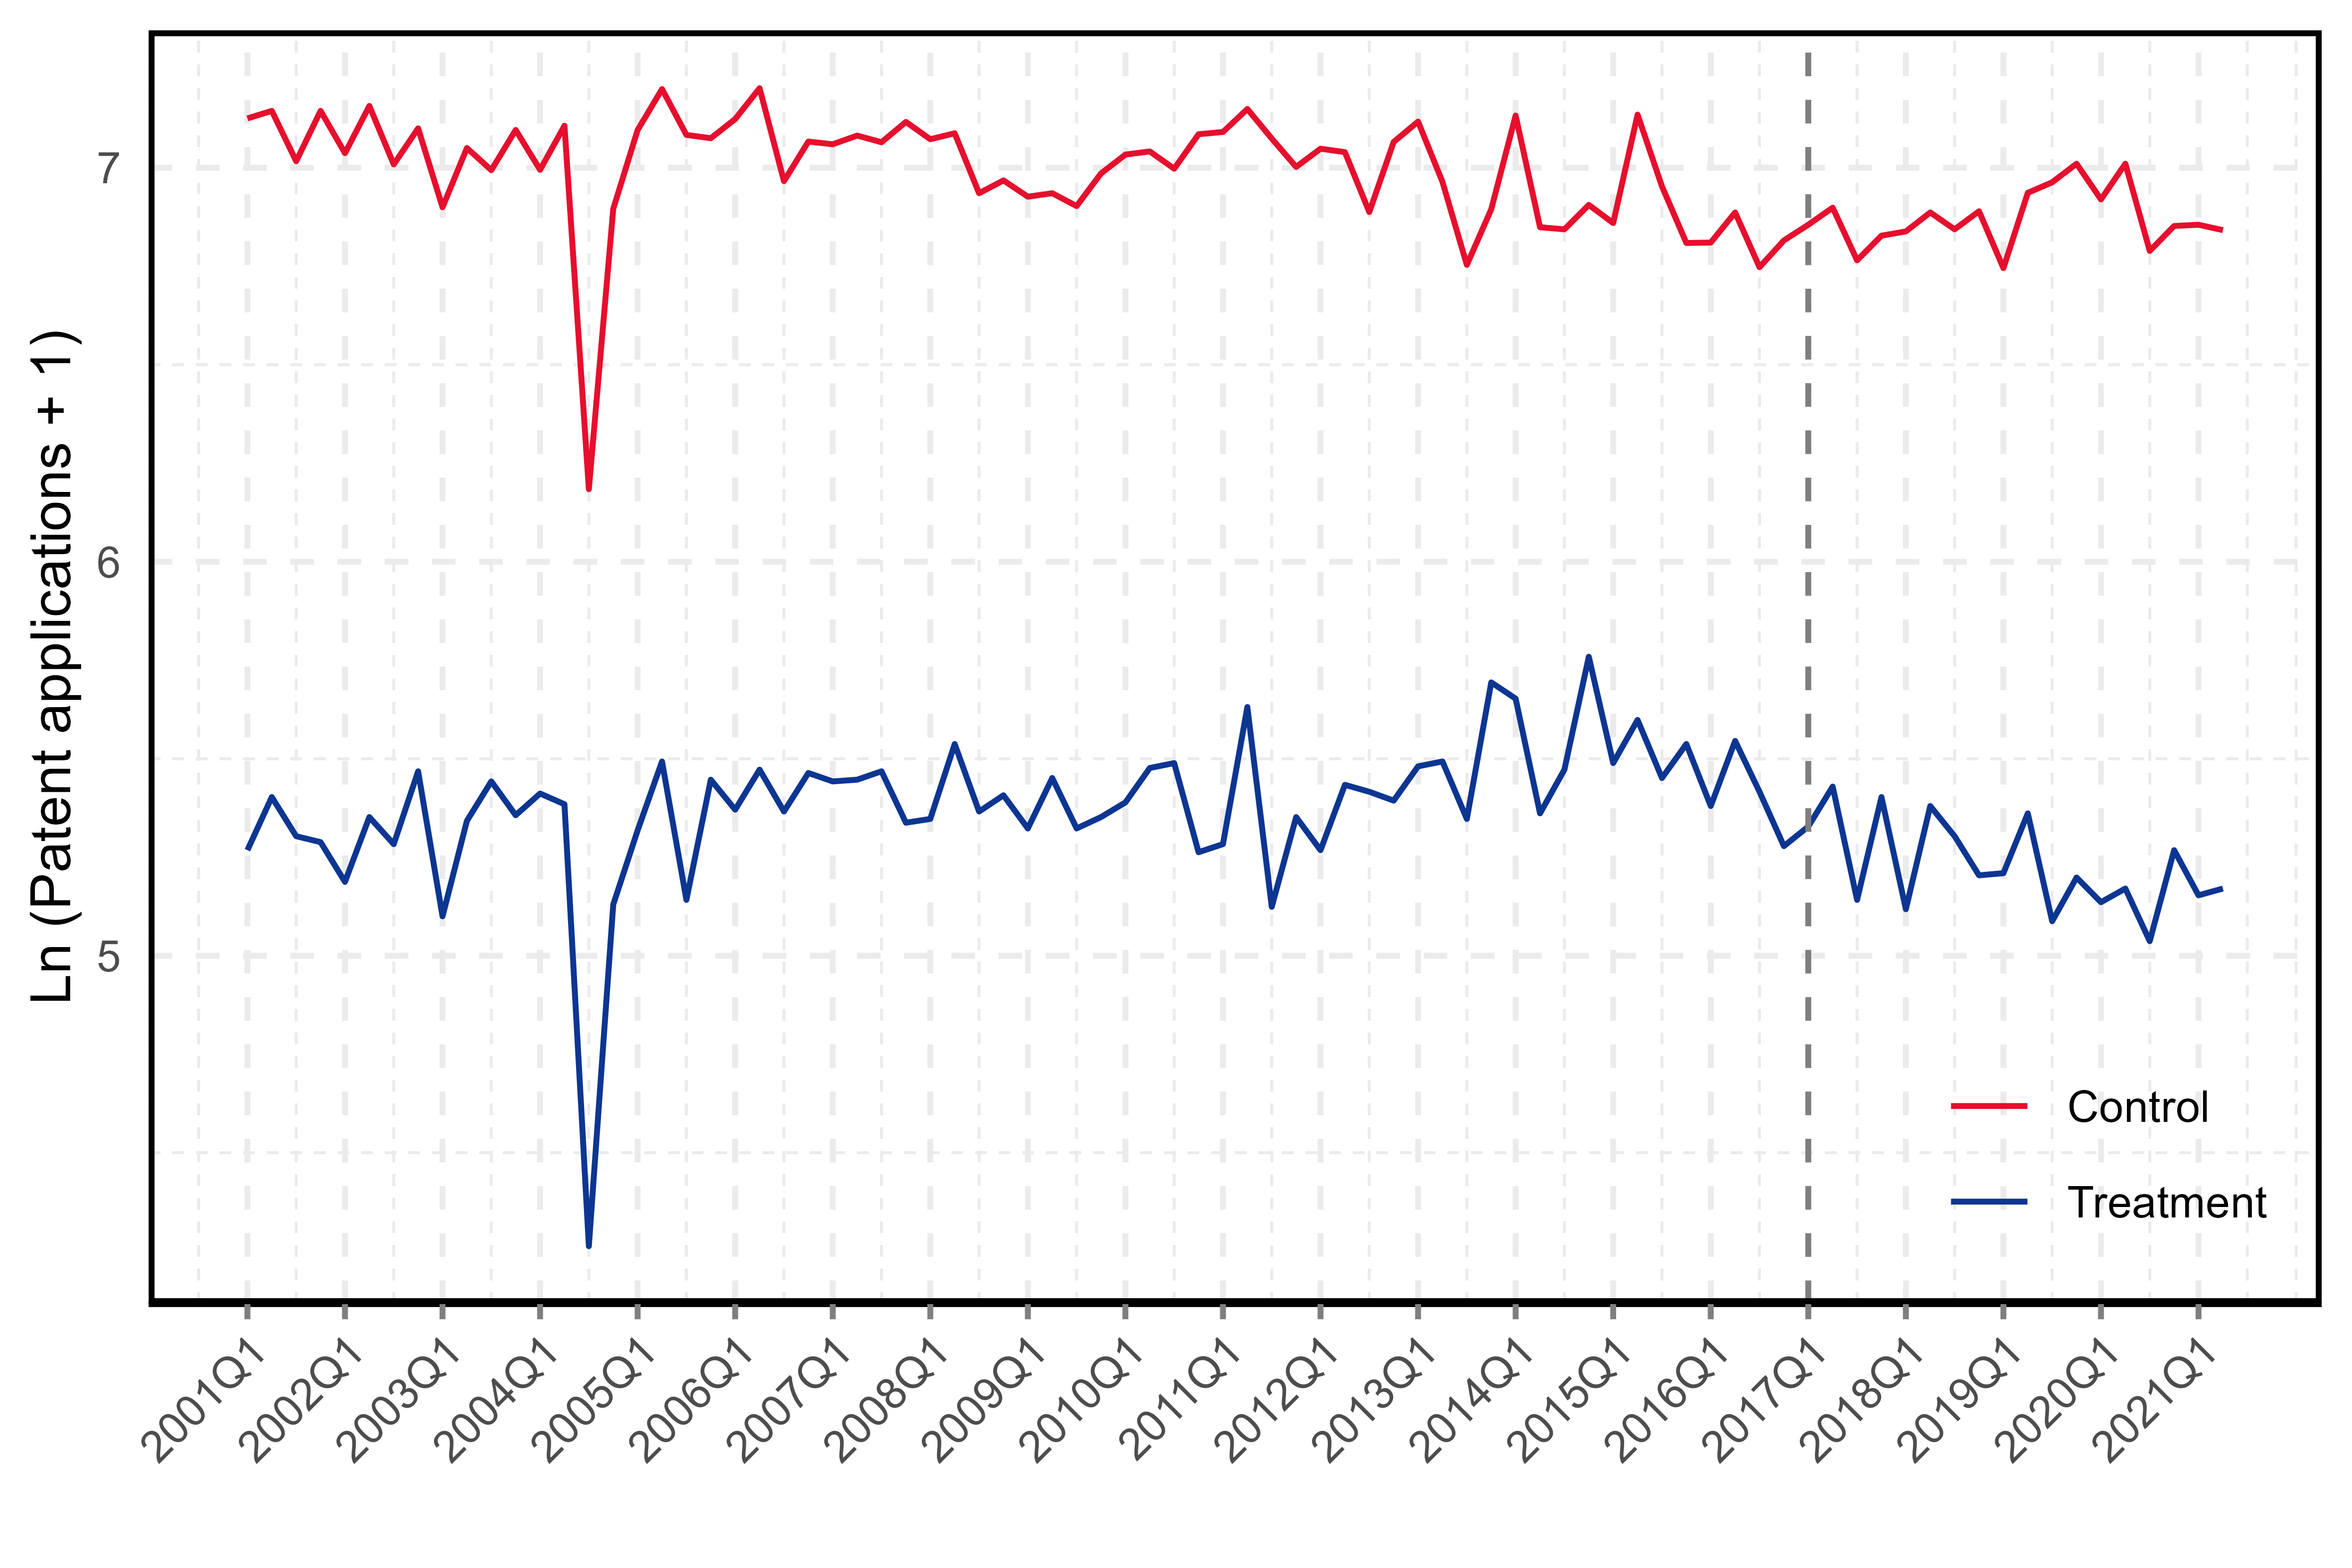
\includegraphics[scale= 0.8]{quarterly_common_trends.png}
    \caption{Grafica}
    \label{fig:figura-control}
\end{figure}

\end{document}
